\chapter{FUNDAMENTOS DO MÉTODO MAGNETOTELÚRICO}

    Proposto com \cite{tikhonov1950determining} e \cite{cagniard1953basic} o método magnetotelúrico usa as fontes passivas\footnote{São fontes de sinal que não dependem de instrumentos artificiais para gerá-la, ou seja, sinais naturais do planeta.} eletromagnéticas do planeta Terra para estudar e mapear a subsuperfície.
    
    Nesta secção será mostrado sucintamente a origem do sinal MT. Entretanto, antes de demonstrar as bases teóricas do método, será descrito brevemente sobre a resistividade elétrica, sendo esse o elemento fundamental para as interpretações lito-geofísicas com base no magnetotelúrico.
        

    \section{Resistividade Elétrica dos Materiais}
    
        
        O método MT usa a resistividade elétrica ($\rho$ [$\Omega m$]) ou o seu inverso, a condutividade elétrica ($\sigma$ [$S$]), para distinguir e estudar a distribuição dos elementos geológicos em subsuperfície. 
        
        A resistividade elétrica é um parâmetro físico intrínseco a cada material. Ela pode ser definida pela oposição do fluxo de corrente elétrica em um material, ou seja, a resistividade elétrica é igual ao campo elétrico sobre a densidade de corrente \cite{eletromag8hayt}:
        
        \begin{equation}
            \label{resis-antes}
            \rho = \dfrac{E}{J}
        \end{equation}

        \noindent Onde, $E$ é a magnitude do campo elétrico em [V/m] e $J$ é a densidade de corrente em [A/m\textsuperscript{2}].
        
        Se o campo elétrico e a corrente elétrica forem constantes, eles podem assumir os seguintes valores:
        
        \begin{equation}
            \label{campo-eletrico}
            E = \frac{\Delta U}{\Delta l}
        \end{equation}
        
        {\footnotesize \noindent
            \begin{table}[H]
                \begin{tabular*}{5cm}{p{0.4cm}p{0.1cm}p{10cm}}
                    {\footnotesize $\Delta U$}  & {\footnotesize $\rightarrow$} & {\footnotesize Diferença de potêncial [V] }\\
                    {\footnotesize $\Delta l$}         & {\footnotesize $\rightarrow$} & {\footnotesize Comprimento do condutor [m]}\\
                \end{tabular*}
            \end{table}}
            
        \noindent e ainda,
        
        \begin{equation}
            \label{densidade-de-corrente}
            J = \frac{i}{A}
        \end{equation}
        
        {\footnotesize \noindent
            \begin{table}[H]
                \begin{tabular*}{1cm}{p{0.05cm}p{0.1cm}p{10cm}}
                    {\footnotesize $i$}  & {\footnotesize $\rightarrow$} & {\footnotesize Corrente Elétrica [A] }\\
                    {\footnotesize $A$}  & {\footnotesize $\rightarrow$} & {\footnotesize Seção transversal do condutor [m\textsuperscript{2}]}\\
                \end{tabular*}
            \end{table}}

        \noindent Substituindo as equações [\ref{campo-eletrico}] e [\ref{densidade-de-corrente}] na equação [\ref{resis-antes}], obtém-se:
        
        \begin{equation}
            \label{resistividade}
            %\rho = \dfrac{\Delta U \, A}{\Delta l \, i}
            \rho = \dfrac{\Delta U}{i} \dfrac{A}{\Delta l}
        \end{equation}

        Utilizando a equação [\ref{resistividade}], pode-se estimar a resistividade elétrica de um material geológico experimentalmente, a partir do arranjo mostrado na Figura \ref{arranjo-resistividade}.

        \begin{figure}[H]
            \caption[Arranjo para obter a resistividade elétrica]{Arranjo para obter experimentalmente a resistividade elétrica de um material geológico.}
                \begin{center}
                    \includegraphics[width=4cm]{texto/figura/resisti_telford.png}
                \end{center}
            \legend{\Fonte{Adaptado \cite{telford}.}}
            \label{arranjo-resistividade}
        \end{figure}
        
        Devido a complexidade físico-químicas dos materiais geológicos, a resistividade elétrica é representada por um intervalo de valores. A Figura \ref{tabela-resis} mostra esses intervalos de valores para alguns tipos de rochas. Entretanto vale ressaltar que os valores podem serem alterados dependendo do contexto geológico. 
        
        \begin{figure}[H]
            \caption{Tabela de resistividade elétrica para materiais geológicos.}
                \begin{center}
                    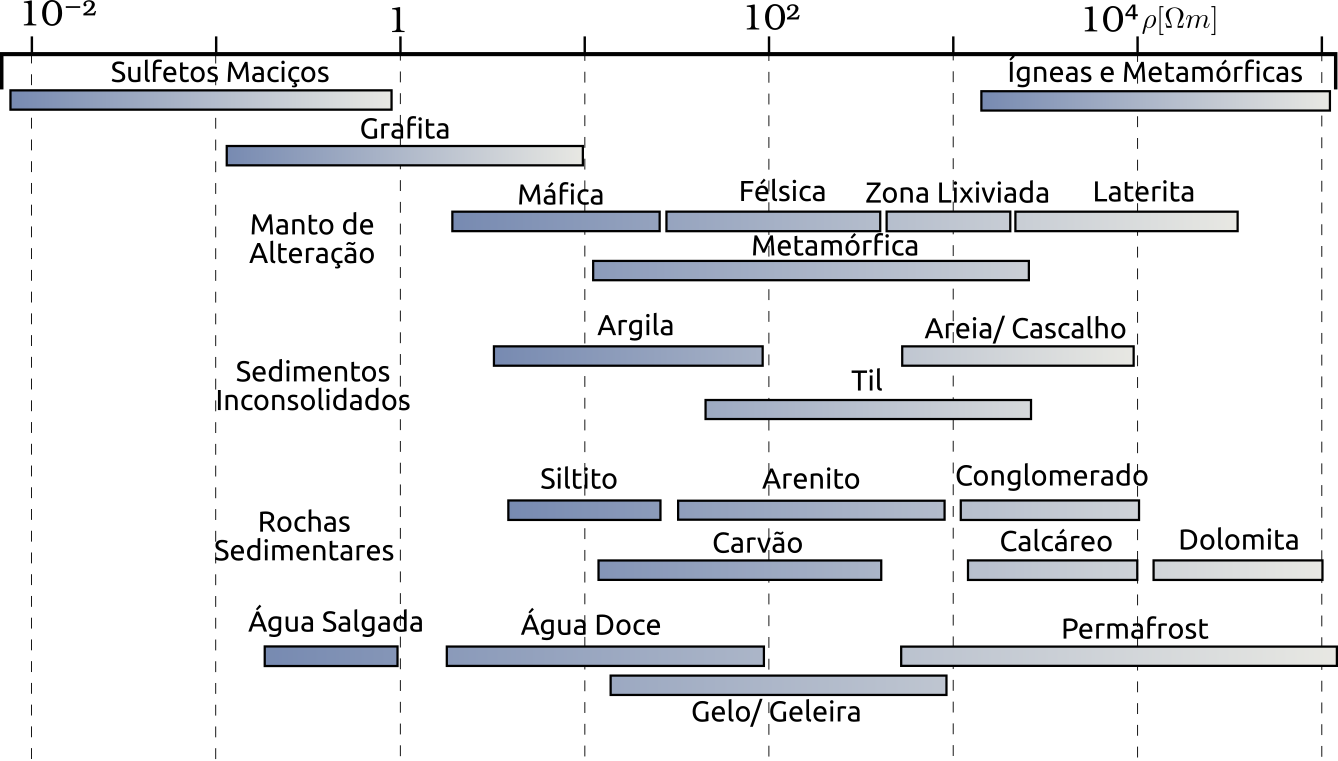
\includegraphics[width=13cm]{texto/figura/resistividade_tabela.png}
                \end{center}
            \legend{\Fonte{Adaptado \cite{palacky}.}}
            \label{tabela-resis}
        \end{figure}
    
    \section{Origem das Correntes Telúricas}
    
        O método MT utiliza-se de um amplo espectro do campo eletromagnético natural terrestre (10\textsuperscript{-4} a 10\textsuperscript{4} Hz) para as sondagens geofísicas. Essa característica permite que  a sondagem magnetotelúrica alcance centenas de quilômetros.
        
        O sinal MT tem sua origem nas ressonâncias de Schumann, nas micropulsações e nas variações diurnas \cite{padua2004estudos}. A figura \ref{sinalmt} mostra a contribuição de cada mecânismo no espectro MT.
        
        \begin{figure}[H]
            \caption{Campo magnético natural e as contribuições das fontes do sinal MT.}
                \begin{center}
                    \includegraphics[width=12cm]{texto/figura/padua04.eps}
                \end{center}
            \legend{\Fonte{Adaptado \cite{padua2004estudos}.}}
            \label{sinalmt}
        \end{figure}
        
        As ressonâncias de Schumann tem sua origem principalmente nas tempestades equatoriais contribuindo para a fonte do sinal MT acima de 1 Hz, as frequências a baixo desse valor, tem origem na interação do vento solar com a magnetosfera, que geram ressonâncias Terra-ionosfera. A contribuição de parte do espectro MT, tambem pode ser explicada pela distorção do formato do campo magnético terrestre causada pelo Sol durante o dia, esse processo é chamado de variação diurna e contribui com a faixa de frequência de 10\textsuperscript{-5} a 10\textsuperscript{-4} Hz. 
        
        
        %\subsection{Ressonâncias de Schumann}
        
        %\subsection{Micropulsações}
        
        %\subsection{Variações Diurnas}   
        
    \section{Resposta do Método Magnetotelúrico}

        O \mt{} assim como outros métodos geofísicos eletromagnéticos, fundamentam-se nas Leis de Maxwell [\ref{lei-max-rotE} -- \ref{lei-max-divD}], pode-se partir das equações estimar os parâmetros físicos para a investigação MT, assim:
        
        \begin{equation}
            \label{lei-max-rotE}
            \rot{E} = - \devpart{\vetor{B}}
        \end{equation}
        \begin{equation}
            \label{lei-max-rotH}
            \rot{H} = \vetor{J} + \devpart{\vetor{D}}
        \end{equation}

        \begin{equation}
            \label{lei-max-divB}
            \nabla \cdot \vetor{B} = 0 
        \end{equation}

        \begin{equation}
            \label{lei-max-divD}
            \nabla \cdot \vetor{D} = \varrho                
        \end{equation}
        
        \noindent Onde,
            
        {\footnotesize \noindent
            \begin{table}[H]
                \begin{tabular*}{1cm}{p{0.05cm}p{0.1cm}p{10cm}}
                    {\footnotesize $\vec{\textrm{E}}$}  & {\footnotesize $\rightarrow$} & {\footnotesize Vetor Campo Elétrico [V/m] }\\
                    {\footnotesize $\vec{\textrm{B}}$}  & {\footnotesize $\rightarrow$} & {\footnotesize Vetor Campo Magnético [T] }\\
                    {\footnotesize $\vec{\textrm{H}}$}  & {\footnotesize $\rightarrow$} & {\footnotesize Vetor Campo Magnetizante [A/m]} \\
                    {\footnotesize $\vec{\textrm{J}}$}  & {\footnotesize $\rightarrow$} & {\footnotesize Vetor Densidade de Corrente [A/m\textsuperscript{2}]} \\
                    {\footnotesize $\vec{\textrm{D}}$}  & {\footnotesize $\rightarrow$} & {\footnotesize Vetor Campo de Deslocamento Elétrico [C/m\textsuperscript{2}]} \\
                    {\footnotesize $\varrho$}           & {\footnotesize $\rightarrow$} & {\footnotesize Densidade de Carga [C/m\textsuperscript{3}]} \\
                    {\footnotesize $t$ }                & {\footnotesize $\rightarrow$} & {\footnotesize Tempo [s]}
                \end{tabular*}
            \end{table}}

        Para os estudos \mt s são feitas as seguintes afirmações, que auxiliam e simplificam o desenvolvimento:
       
        \begin{quote}
            A Terra comporta-se como um condutor ôhmico e um semi-espaço isotrópico.
        \end{quote}
        
        Podemos utilizar, partindo dessas característica e atrelado a um campo eletromagnético pouco intenso as seguintes relações constitutivas:
        \begin{equation}
         \vetor{B} = \mu \vetor{H}
        \end{equation}
        
        \begin{equation}
         \vetor{D} = \varepsilon \vetor{E}
        \end{equation}
        
        \begin{equation}
         \vetor{J} = \sigma \vetor{E}
        \end{equation}

        {\footnotesize \noindent
            \begin{table}[H]
                \begin{tabular*}{1cm}{p{0.05cm}p{0.1cm}p{10cm}}
                    {\footnotesize $\mu$}          & {\footnotesize $\rightarrow$} & {\footnotesize Permeabilidade Magnética [H/m] }\\
                    {\footnotesize $\varepsilon$}  & {\footnotesize $\rightarrow$} & {\footnotesize Permissividade Elétrica [F/m] }\\
                    {\footnotesize $\sigma$}       & {\footnotesize $\rightarrow$} & {\footnotesize Condutividade Elétrica [S/m]} \\
                \end{tabular*}
            \end{table}}

        Cada coeficiente das relações constitutivas funcionam como tensores, variantes no tempo, para meios anisotrópicos. Para o estudo abordado e seguindo a afirmação, onde a Terra torna-se um meio isotrópico, isso implica que os tensores, $\mu$ e $\varepsilon$ são estáticos e assumem os valores referência para o vácuo:
        
        \begin{quote}
            \begin{enumerate}
                \item[$\mu$] $=$ \basedez{1{,}2566}{-6} H/m
                \item[$\varepsilon$] $=$ \basedez{8{,}85}{-12} F/m
            \end{enumerate}
        \end{quote}
        
        Utilizando as equações constitutivas podemos reescrever as equações \ref{lei-max-rotE} e \ref{lei-max-rotH}:
        
        {\setlength\arraycolsep{2pt}
        \begin{eqnarray}
            \label{rotEconstH}
            \rot{E} &=& - \devpart{\vetor{B}}; \qquad \vetor{B} = \mu \vetor{H} \nonumber \\
            \rot{E} &=& - \mu \devpart{\vetor{H}}
        \end{eqnarray}}

        {\setlength\arraycolsep{2pt}
        \begin{eqnarray}
            \label{rotHconstE}
            \rot{H} &=& \vetor{J} + \devpart{\vetor{D}}; \qquad \vetor{J} = \sigma \vetor{E} \quad \textrm{e} \quad \vetor{D} = \varepsilon \vetor{E}\nonumber \\
            & &\rot{H} =  \sigma \vetor{E} + \varepsilon \devpart{\vetor{E}}
        \end{eqnarray}}
        
        Na faixa da sondagem MT a Terra comporta-se como um condutor ôhmico, isso implica que o meio não possuem cargas livres, logo $\varrho \simeq 0$. 
        
        Para os campos pode ser assumida uma dependência temporal harmônica dada por $e^{- \imath \omega t}$, que pode ser decomposta em vários harmônicos pela transformada de Fourier, onde $t$ é o tempo e $\omega$ a frequência angular. 
    
        Portando as equações: \ref{rotEconstH}, \ref{rotHconstE}, \ref{lei-max-divB} e \ref{lei-max-divD}, podem ser reescritas como:
        
        \begin{equation}
            \label{rotEconstHreescrito}
            \rot{E} = \imath \omega \mu \vetor{H}           
        \end{equation}
        
        \begin{equation}
            \label{rotHconstEreescrito}
            \rot{H} = (\imath \omega \varepsilon + \sigma) \vetor{E}
        \end{equation}
        
        \begin{equation}
            \nabla \cdot \vetor{H}  = 0
        \end{equation}

        \begin{equation}
            \nabla \cdot \vetor{E} = 0
        \end{equation}

        Aplicando o rotacional na equação \ref{rotHconstEreescrito}, obtemos:
         
        \begin{equation}
            \label{rotrotH}
            \nabla \times \nabla \times \vetor{H} = (\imath \omega \varepsilon + \sigma) \rot{E}
        \end{equation}

        Comparando a equação \ref{rotrotH} com a equação \ref{rotEconstHreescrito}, pode-se reescreve-la como:
        
        {\setlength\arraycolsep{2pt}
        \begin{eqnarray}
            \label{preHk}
            \nabla \times \nabla \times \vetor{H} &=& (\imath \omega \varepsilon + \sigma) \rot{E}; \qquad \rot{E} = \imath \omega \mu \vetor{H} \nonumber \\
            & &\nabla \times \nabla \times \vetor{H} = \imath \omega \mu (\imath \omega \varepsilon + \sigma) \vetor{H}            
        \end{eqnarray}}
        
        Pode-se expressar a equação \ref{preHk} usando a seguinte identidade vetorial:
        
        \begin{equation}
            \nabla \times \nabla \times \vetor{A} = \nabla \nabla \cdot \vetor{A} - \nabla^2 \vetor{A} 
        \end{equation}

        \noindent Portanto:
        
        {\setlength\arraycolsep{2pt}
        \begin{eqnarray}
            \label{difH}
            \nabla \nabla \cdot \vetor{H} - \nabla^2 \vetor{H} & = & \imath \omega \mu (\imath \omega \varepsilon + \sigma) \vetor{H} \nonumber \\
            \nabla (\nabla \cdot \vetor{H}) - \nabla^2 \vetor{H} & = & \vetor{H}[\cancelto{\kappa^2}{\imath \omega \mu (\imath \omega \varepsilon + \sigma)}] \nonumber \\
            \nabla (\cancelto{0}{\nabla \cdot \vetor{H}}) - \nabla^2 \vetor{H} & = & \kappa^2 \vetor{H} \nonumber \\
            \nabla^2 \vetor{H} + \kappa^2 \vetor{H} & = &  0; \qquad \kappa^2 = \imath \omega \mu (\imath \omega \varepsilon + \sigma)
        \end{eqnarray}}        
        
        Considerando um condutor ôhmico ($\sigma \gg \omega \varepsilon$), assim:
        \begin{equation}
            \label{kappaquad}
            \kappa^2 = \imath \omega \mu \sigma
        \end{equation}
        
        \noindent Onde, $\kappa^2$ é o módulo do vetor de onda ($\vetor{k}$).
        
        A equação \ref{kappaquad} pode ser expressa seguindo a definição, como:
        
        {\setlength\arraycolsep{2pt}
        \begin{eqnarray}
            \kappa & = & \sqrt{\imath \omega \mu \sigma}; \quad \imath = e^{\imath \frac{\pi}{2}} \nonumber \\
            \kappa & = & \sqrt{\omega \mu \sigma} \sqrt{e^{\imath \frac{\pi}{2}}} \nonumber \\
            \kappa & = & \sqrt{\omega \mu \sigma} e^{\imath \frac{\pi}{4}}; \quad e^{\imath \frac{\pi}{4}} = \sqrt{1/2} (1 + \imath) \nonumber \\
            \kappa & = & \sqrt{\dfrac{\omega \mu \sigma}{2}} (1 + \imath) \nonumber \\
            \kappa & = & \dfrac{(1 + \imath)}{\delta}
        \end{eqnarray}} 
        
        \noindent Onde,
        
        \begin{equation}
            \label{shin-depth}
            \delta_\omega = \sqrt{\dfrac{2 \rho}{\omega \mu}} \longrightarrow \delta_f \approx 500  \sqrt{\frac{\rho_a}{f}}
        \end{equation}
        
        A equação \ref{shin-depth} é chamada de \en{skin-depth} (Espessura pelicular), ela representa a profundidade de penetração da onda eletromagnética em um meio condutor.
        A partir da equação são mapeadas as litologias em subsuperfície. Porém a resistividade ($\rho$) representa todo o pacote de rochas em subsuperfície, portanto, adota-se o termo resistividade aparente ($\rho_a$) para a mesma. A resistividade efetiva ($\rho$) pode ser obtida a partir do processo de inversão geofísica (não tratado neste trabalho).        

        O meio geológico influencia diretamente a profundidade de investigação, a figura \ref{fig-skin-depth} mostra que para uma mesma frequência, ela pode representar valores diferentes de profundidade, variando o meio em subsuperfície, isso é representado por $\rho$. Os meios mais resistivos geram profundidade maiores, já meios condutivos diminuem a profundidade. Esse fenômeno é importante porque, ao interpretar as seções lito-geofísicas, é comum estudar contextos de bacias sedimentares (meio condutivo) em contado com contextos cristalinos (meio resistivo), a atenção deve-se voltar para o fato de que um mesmo período em função de $\rho$ pode representar duas profundidades diferentes, estando a estação em cima do contexto sedimentar ou em cima do contexto cristalino. 
        
        \begin{figure}[H]
            \caption[Gráfico do \en{skin-depth}]{Gráfico do \en{skin-depth} em função da frequência [Hz], variando a resistividade do meio}
            \begin{center}
                \includegraphics[width=10cm]{texto/figura/skin-depth.png}
            \end{center}
            \legend{\Fonte{\oautor.}}
            \label{fig-skin-depth}
        \end{figure}
        
    \section{Impedância Eletromagnética}
        
        Baseado na fundamentação teórica apresentada a seção anterior, o MT busca obter a resistividade aparente em função da profundidade. A partir da solução da equação \ref{difH} e da sua análoga para o campo $\vetor{E}$, onde são dadas por:
        
        \begin{equation}
            \label{soluH}
            \vetor{H}_{(\vetor{r})} = \vetor{H} e^{-\vetor{k} \cdot \vetor{r}}
        \end{equation}

        \begin{equation}
            \label{soluE}
            \vetor{E}_{(\vetor{r})} = \vetor{E} e^{-\vetor{k} \cdot \vetor{r}}
        \end{equation}

        %\noindent Onde $\vetor{k}$ é o vetor de onda, cujo o módulo é definido por $\kappa$ na equação \ref{kappaquad}.
        
        Substituindo a equação \ref{soluH} e \ref{soluE} em \ref{rotHconstEreescrito}, temos:
        
        {\setlength\arraycolsep{2pt}
        \begin{eqnarray}
            \label{HEpossolu}
            \nabla \times \vetor{H}e^{-\vetor{k} \cdot \vetor{r}} & = & (\imath \omega \varepsilon + \sigma) \vetor{E}e^{-\vetor{k} \cdot \vetor{r}}; \quad \sigma \gg \imath \omega \varepsilon \ \nonumber \\
            \nabla \times \vetor{H}e^{-\vetor{k} \cdot \vetor{r}} & = & \sigma \vetor{E}e^{-\vetor{k} \cdot \vetor{r}}; \quad \sigma = \dfrac{\kappa^2}{\imath \omega \mu} \nonumber \\
            \nabla \times \vetor{H}e^{-\vetor{k} \cdot \vetor{r}} & = &\dfrac{\kappa^2}{\imath \omega \mu} \vetor{E}e^{-\vetor{k} \cdot \vetor{r}}
        \end{eqnarray}} 
        
        \noindent Usando as identidades:
        
        \begin{equation}
            \nabla (e^{-\vetor{k} \cdot \vetor{r}}) = - e^{-\vetor{k} \cdot \vetor{r}} \vetor{k}
        \end{equation}

        \begin{equation}
            \nabla \times \vetor{C}(f_{(\vetor{r})}) = - \vetor{C} \times \nabla f_{(\vetor{r})} 
        \end{equation}
        
        Pode-se reescrever a equação \ref{HEpossolu}:
        
        {\setlength\arraycolsep{2pt}
        \begin{eqnarray}
            \label{EZHvetor}
            - \vetor{H} \times (- e^{-\vetor{k} \cdot \vetor{r}} \vetor{k}) = \dfrac{\kappa^2}{\imath \omega \mu} \vetor{E}e^{-\vetor{k} \cdot \vetor{r}} \nonumber \\
            \cancelto{}{e^{-\vetor{k} \cdot \vetor{r}}} (\vetor{H} \times \vetor{k}) = \cancelto{}{e^{-\vetor{k} \cdot \vetor{r}}} \dfrac{\kappa^2}{\imath \omega \mu} \vetor{E}\nonumber \\
            \vetor{E} = \dfrac{\imath \omega \mu}{\kappa^2} \vetor{H} \times \vetor{k} \nonumber \\
            \vetor{E} = \dfrac{\imath \omega \mu}{\kappa} \vetor{H} \times \dfrac{\vetor{k}}{\kappa}
        \end{eqnarray}} 
        
        \noindent A relação $\vetor{k}/\kappa$ é o versor de $\vetor{k}$ ou  $\hat{\unitario{k}}$, representando a ortogonalidade entre $\vetor{H}$ e $\vetor{E}$.
        
        A partir da equação anterior pode ser definido que $Z = \imath \omega \mu / \kappa$, esta definição é conhecida como impedância intrínseca do meio ou impedância eletromagnética, também pode ser representada da seguinte forma:
        
        \begin{equation}
            Z = \dfrac{|\vetor{E}|}{|\vetor{H}|} = \dfrac{\imath \omega \mu}{\kappa} = \sqrt{\omega \mu \rho} e^{\imath \frac{\pi}{4}}
        \end{equation}
        
        A impedância eletromagnética ($Z$) pode ser decomposta em função das componentes de $\vetor{E}$ e $\vetor{H}$, representada na forma matricial:
        
        \begin{equation}
            \label{tensor-impe}
            \left (\begin{array}{c}
                \textrm{E}_x\\
                \textrm{E}_y
                    \end{array}\right)
                =
            \left (\begin{array}{cc}
                \textrm{Z}_{xx} & \textrm{Z}_{xy}\\
                \textrm{Z}_{yx} & \textrm{Z}_{yy}
                    \end{array}\right)
            \left (\begin{array}{c}
                \textrm{H}_x\\
                \textrm{H}_y
                    \end{array}\right)
	    \end{equation}
	    
	    O método MT, então, obtém a resistividade aparente a partir da impedância eletromagnética, e atribui a ela uma profundidade, onde pode ser definida pela função de \en{skin-depth} (equação \ref{shin-depth}).          
